\graphicspath{ {images/} }

\newcommand{\Real}{\mathbb{R}}
\newcommand{\Int}{\mathbb{Z}}

\newcommand{\henc}{\bh^{\text{enc}}}
\newcommand{\hencfw}[1]{\overrightarrow{\henc_{#1}}}
\newcommand{\hencbw}[1]{\overleftarrow{\henc_{#1}}}

\newcommand{\cenc}{\bc^{\text{enc}}}
\newcommand{\cencfw}[1]{\overrightarrow{\cenc_{#1}}}
\newcommand{\cencbw}[1]{\overleftarrow{\cenc_{#1}}}

\newcommand{\hdec}{\bh^{\text{dec}}}

\newcommand{\cdec}{\bc^{\text{dec}}}

\newcommand{\AK}[1]{{\color{blue} {\bf (AK: #1)}}}


\lstset{basicstyle=\ttfamily,columns=flexible,numbers=none}

\titledquestion{Pretrained Transformer models and knowledge access}[35]
\label{sec:char_enc}

You'll train a Transformer to perform a task that involves accessing knowledge about the world --- knowledge which isn't provided via the task's training data (at least if you want to generalize outside the training set). You'll find that it more or less fails entirely at the task.
You'll then learn how to pretrain that Transformer on Wikipedia text that contains world knowledge, and find that finetuning that Transformer on the same knowledge-intensive task enables the model to access some of the knowledge learned at pretraining time.
You'll find that this enables models to perform considerably above chance on a held out development set.


The code you're provided with is a fork of Andrej Karpathy's \href{https://github.com/karpathy/minGPT}{\mingpt}.
It's nicer than most research code in that it's relatively simple and transparent.
The ``GPT'' in \mingpt refers to the Transformer language model of OpenAI, originally described in \href{https://s3-us-west-2.amazonaws.com/openai-assets/research-covers/language-unsupervised/language_understanding_paper.pdf}{this paper} \cite{radford2018improving}.

As in previous assignments, you will want to develop on your machine locally, then run training on Azure/Colab. You can use the same conda environment from previous assignments for local development, and the same process for training on a GPU.\footnote{See \href{https://docs.google.com/document/d/11kRyfClhTi4-MC1feWWCMI31fHpTzddASsDa48_Dd9E/edit?usp=sharing}{CS224n Azure Guide} for a refresher on Azure.}
You'll need around 5 hours for training, so budget your time accordingly! We have provided a sample Colab with the the commands that require GPU training. \textbf{Note that dataset multi-processing can fail on local machines without GPU, so to debug locally, you might have to change \texttt{num\_workers} to 0.}

Your work with this codebase is as follows:
\begin{parts}
\part[0]
\textbf{Check out the demo.}\\
In  the \texttt{mingpt-demo/} folder is a Jupyter notebook \texttt{play\_char.ipynb} that trains and samples from a Transformer language model.
Take a look at it (locally on your computer) to get somewhat familiar with how it defines and trains models.
Some of the code you're writing below will be inspired by what you see in this notebook.

Note that you do not have to write any code or submit written answers for this part.



\part[0] \textbf{Read through \texttt{NameDataset} in \texttt{src/dataset.py}, our dataset for reading name-birthplace pairs.}\\
The task we'll be working on with our pretrained models is attempting to access the birth place of a notable person, as written in their Wikipedia page.
We'll think of this as a particularly simple form of question answering:
\begin{quote}
    \textit{Q: Where was \textit{[person]} born?}\\
    \textit{A: [place]}
\end{quote}
From now on, you'll be working with the \texttt{src/} folder. \textbf{The code in \texttt{mingpt-demo/} won't be changed or evaluated for this assignment.}
In \texttt{dataset.py}, 
you'll find the the class \texttt{NameDataset}, which reads a TSV (tab-separated values) file of name/place pairs and produces examples of the above form that we can feed to our Transformer model.


To get a sense of the examples we'll be working with, if you run the following code, it'll load your \texttt{NameDataset} on the training set \texttt{birth\_places\_train.tsv} and print out a few examples.
\begin{lstlisting}[language=bash]
    python src/dataset.py namedata 
\end{lstlisting}

Note that you do not have to write any code or submit written answers for this part.

\part[0] \textbf{Implement finetuning (without pretraining).}\\
Take a look at \texttt{run.py}. It has some skeleton code specifying flags you'll eventually need to handle as command line arguments.
In particular, you might want to \textit{pretrain}, \textit{finetune}, or \textit{evaluate} a model with this code. For now, we'll focus on the finetuning function, in the case without pretraining.

Taking inspiration from the training code in the \texttt{play\_char.ipynb} file, write code to finetune a Transformer model on the name/birthplace dataset, via examples from the \texttt{NameDataset} class. For now, implement the case without pretraining (i.e. create a model from scratch and train it on the birthplace prediction task from part (b)). You'll have to modify two sections, marked \texttt{[part c]} in the code: one to initialize the model, and one to finetune it. Note that you only need to initialize the model in the case labeled ``vanilla'' for now (later in section (g), we will explore a model variant).
Use the hyperparameters for the \texttt{Trainer} specified in the \texttt{run.py} code.

Also take a look at the \textit{evaluation} code which has been implemented for you. It samples predictions from the trained model and calls \texttt{evaluate\_places()} to get the total percentage of correct place predictions. You will run this code in part (d) to evaluate your trained models.

This is an intermediate step for later portions, including Part~\ref{part_predictions_nopretraining}, which contains commands you can run to check your implementation. No written answer is required for this part.

\part[5] \label{part_predictions_nopretraining} \textbf{Make predictions (without pretraining).}\\ 
Train your model on \texttt{birth\_places\_train.tsv}, and evaluate on \texttt{birth\_dev.tsv}. Specifically, you should now be able to run the following three commands:
\begin{lstlisting}[language=bash, basicstyle=\small\ttfamily]
# Train on the names dataset
python src/run.py finetune vanilla wiki.txt \
        --writing_params_path vanilla.model.params \
        --finetune_corpus_path birth_places_train.tsv
        
# Evaluate on the dev set, writing out predictions
python src/run.py evaluate vanilla wiki.txt  \
        --reading_params_path vanilla.model.params \
        --eval_corpus_path birth_dev.tsv \
        --outputs_path vanilla.nopretrain.dev.predictions
        
# Evaluate on the test set, writing out predictions
python src/run.py evaluate vanilla wiki.txt  \
        --reading_params_path vanilla.model.params \
        --eval_corpus_path birth_test_inputs.tsv \
        --outputs_path vanilla.nopretrain.test.predictions
\end{lstlisting}

Training will take less than 10 minutes (on Azure).  Report your model's accuracy on the dev set (as printed by the second command above). Similar to assignment 4, we also have Tensorboard logging in assignment 5 for debugging. It can be launched using \texttt{tensorboard --logdir expt/}.  Don't be surprised if it is well below 10\%; we will be digging into why in Part 3. As a reference point, we want to also calculate the accuracy the model would have achieved if it had just predicted ``London'' as the birth place for everyone in the dev set. Fill in \texttt{london\_baseline.py} to calculate the accuracy of that approach and report your result in your write-up. You should be able to leverage existing code such that the file is only a few lines long. 

\ifans{
        \begin{itemize}
                \item \textbf{Dev accuracy: } Correct: 7.0 out of 500.0: 1.4\%
                \item \textbf{London baseline: } Correct: 25.0 out of 500.0: 5.0\%
        \end{itemize}
}


\part[10]\textbf{Define a \textit{span corruption} function for pretraining.}\\
In the file \texttt{src/dataset.py}, implement the \texttt{\_\_getitem\_\_()} function for the dataset class \\ \texttt{CharCorruptionDataset}.
Follow the instructions provided in the comments in \texttt{dataset.py}.
Span corruption is explored in the \href{https://arxiv.org/pdf/1910.10683.pdf}{T5 paper} \cite{raffel2020exploring}.
It randomly selects spans of text in a document and replaces them with unique tokens (noising).
Models take this noised text, and are required to output a pattern of each unique sentinel followed by the tokens that were replaced by that sentinel in the input.
In this question, you'll implement a simplification that only masks out a single sequence of characters.

This question will be graded via autograder based on whether your span corruption function implements some basic properties of our spec.
We'll instantiate the \texttt{CharCorruptionDataset} with our own data, and draw examples from it.

To help you debug, if you run the following code, it'll sample a few examples from your \\ \texttt{CharCorruptionDataset} on the pretraining dataset \texttt{wiki.txt} and print them out for you.
\begin{lstlisting}[language=bash]
    python src/dataset.py charcorruption
\end{lstlisting}

No written answer is required for this part.

\part[10] \textbf{Pretrain, finetune, and make predictions. Budget 2 hours for training.}\\
Now fill in the \textit{pretrain} portion of \texttt{run.py}, which will pretrain a model on the span corruption task. Additionally, modify your \textit{finetune} portion to handle finetuning in the case \textit{with} pretraining. In particular, if a path to a pretrained model is provided in the bash command, load this model before finetuning it on the birthplace prediction task.
Pretrain your model on \texttt{wiki.txt} (which should take approximately two hours), finetune it on \texttt{NameDataset} and evaluate it. Specifically, you should be able to run the following four commands:
(Don't be concerned if the loss appears to plateau in the middle of pretraining; it will eventually go back down.)
\begin{lstlisting}[language=bash]
# Pretrain the model
python src/run.py pretrain vanilla wiki.txt \
        --writing_params_path vanilla.pretrain.params
        
# Finetune the model
python src/run.py finetune vanilla wiki.txt \
        --reading_params_path vanilla.pretrain.params \
        --writing_params_path vanilla.finetune.params \
        --finetune_corpus_path birth_places_train.tsv
        
# Evaluate on the dev set; write to disk
python src/run.py evaluate vanilla wiki.txt  \
        --reading_params_path vanilla.finetune.params \
        --eval_corpus_path birth_dev.tsv \
        --outputs_path vanilla.pretrain.dev.predictions
        
# Evaluate on the test set; write to disk
python src/run.py evaluate vanilla wiki.txt  \
        --reading_params_path vanilla.finetune.params \
        --eval_corpus_path birth_test_inputs.tsv \
        --outputs_path vanilla.pretrain.test.predictions
\end{lstlisting}

Report the accuracy on the dev set (printed by the third command above). We expect the dev accuracy will be at least 10\%, and will expect a similar accuracy on the held out test set.

\begin{figure}[h]
        \centering
        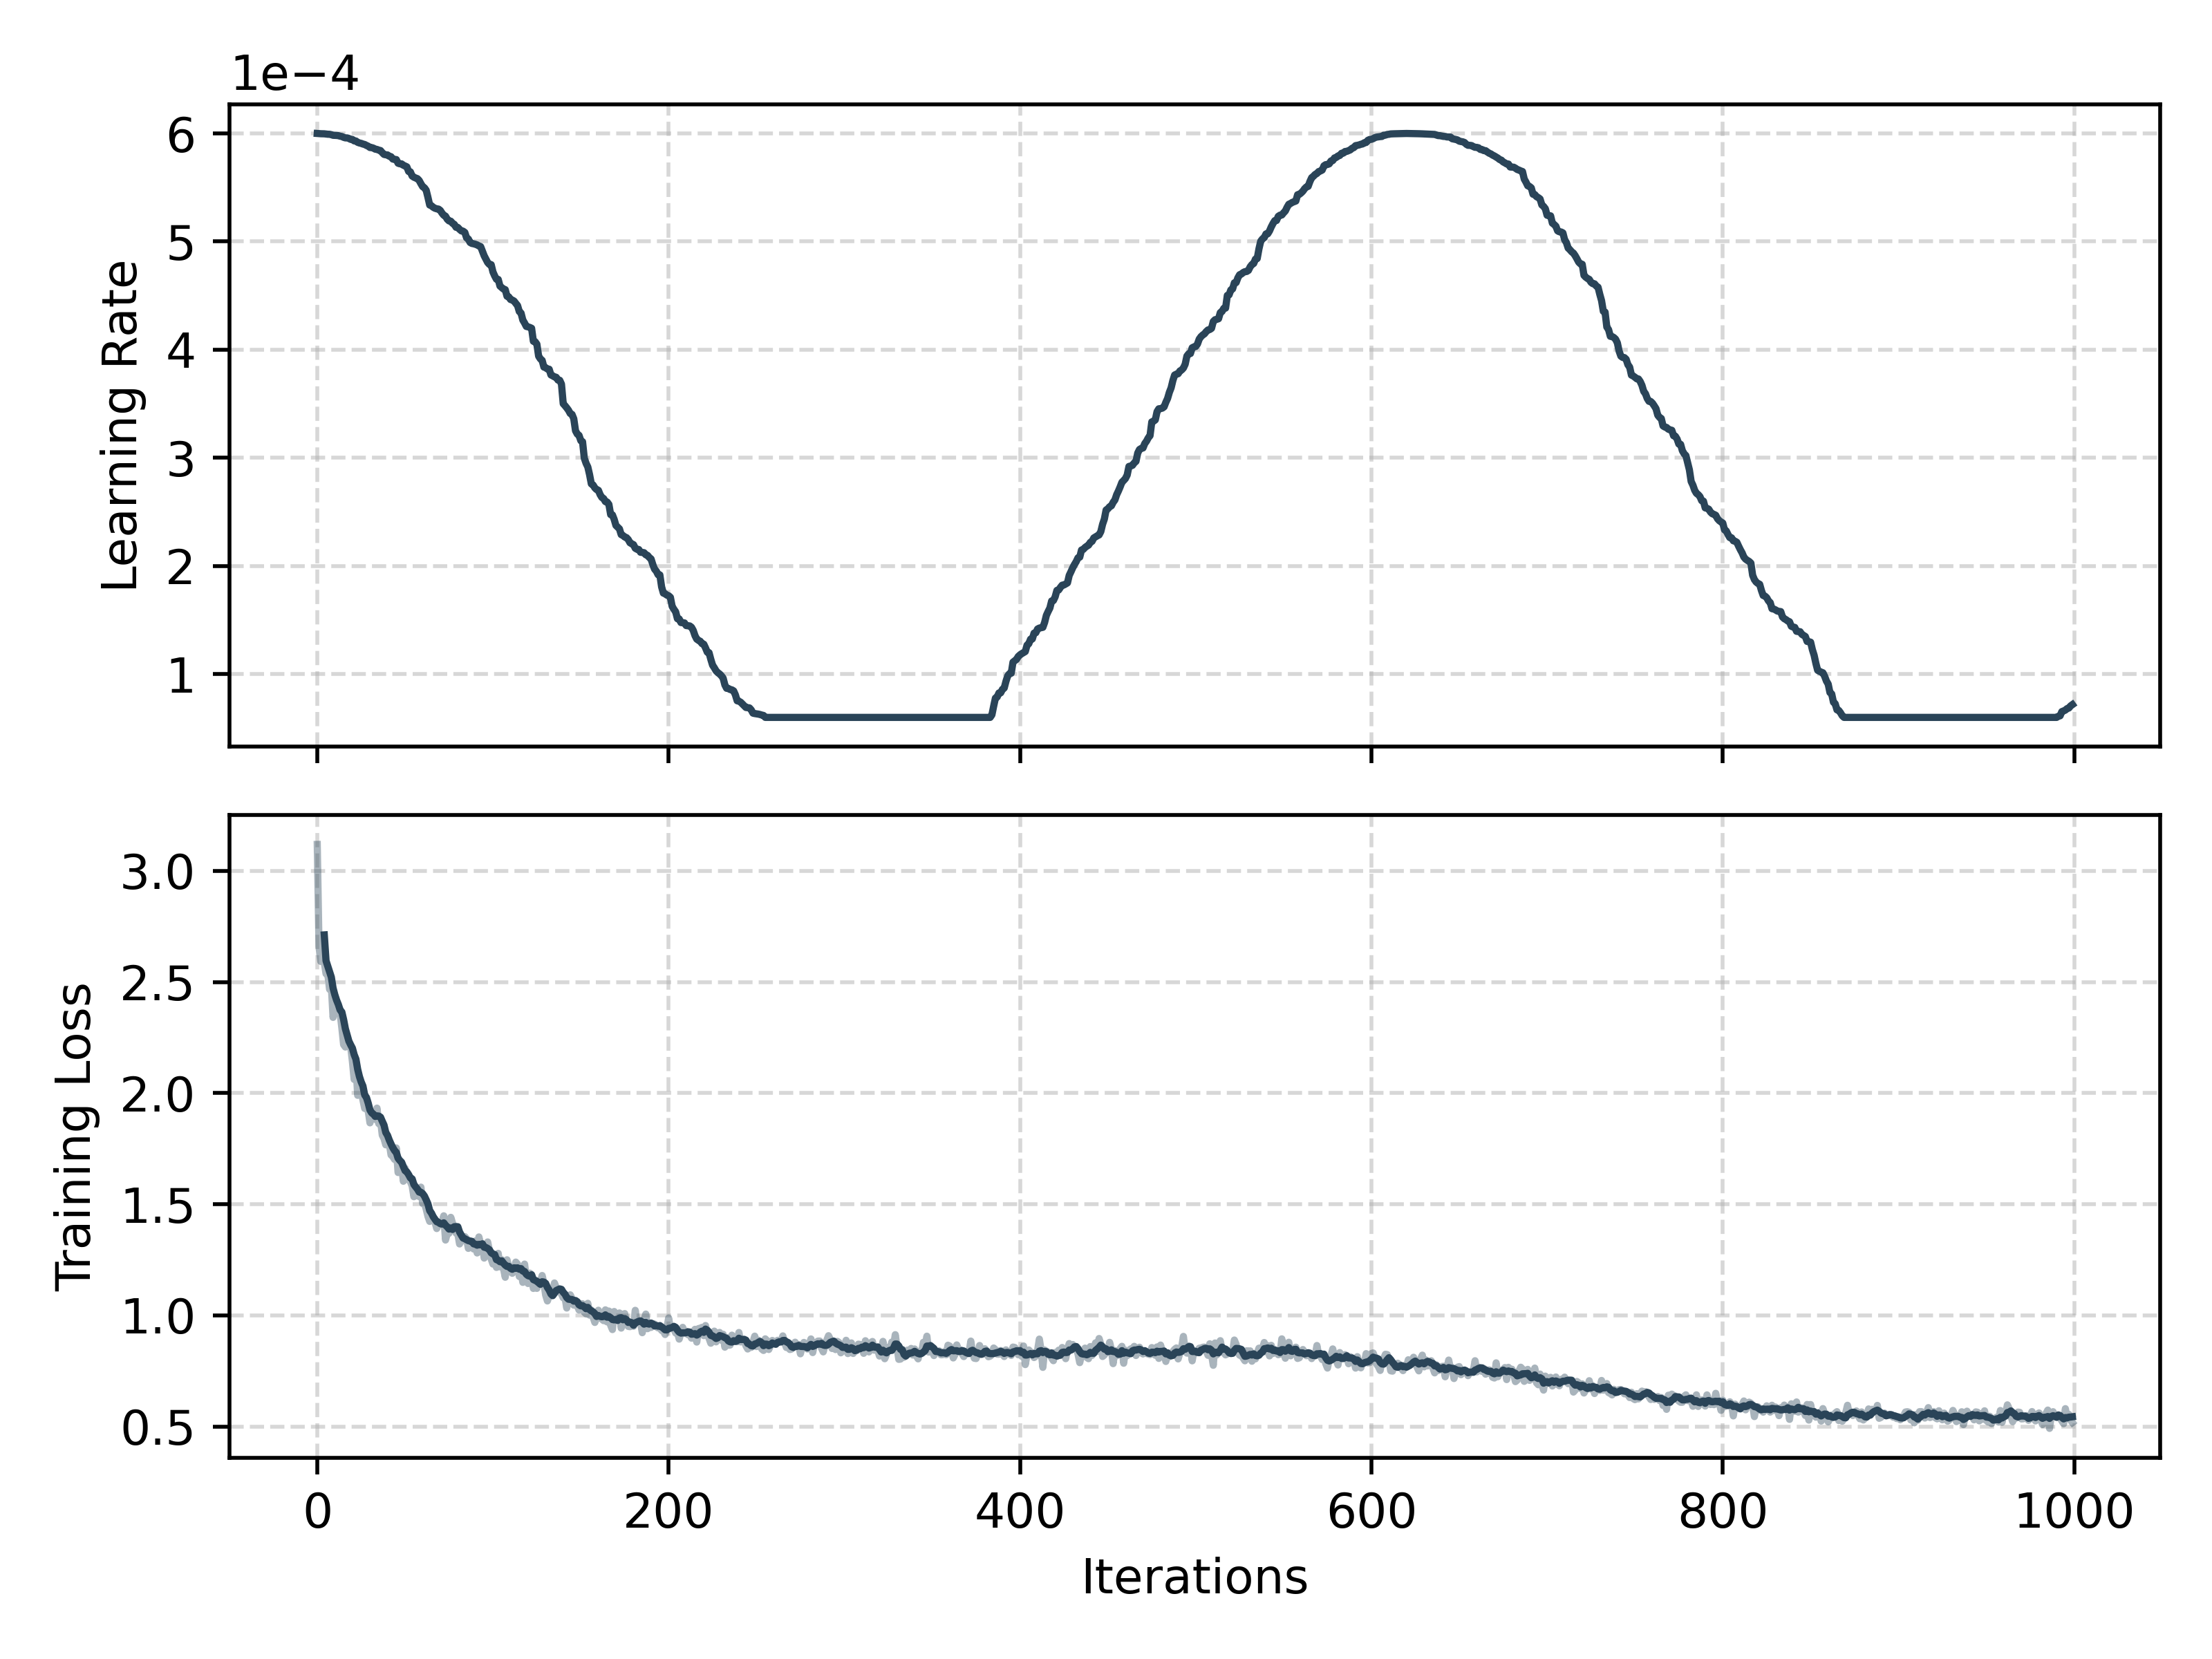
\includegraphics[width=0.5\textwidth]{../code/vanilla_training_process.png}
        \caption{vanilla training process}
        \label{fig:vanilla_training_process}
\end{figure}

\ifans{
        Correct: 65.0 out of 500.0: 13.0\%
}


\part[10] \textbf{Research! Write and try out a more efficient variant of Attention (Budget 2 hours for pretraining!)}\\

We'll now go to changing the Transformer architecture itself -- specifically the first and last transformer blocks.
The transformer model uses a self-attention scoring function based on dot products, this involves a rather intensive computation that's quadratic in the sequence length. This is because the dot product between $\ell^2$ pairs of word vectors is computed in each computation, where $\ell$ is the sequence length. If we can reduce the length of the sequence passed on the self-attention module, we should observe significant reduction in compute. For example, if we develop a technique that can reduce the sequence length to half, we can save around 75\% of the compute time!

PerceiverAR~\cite{hawthorne2022perceiver} proposes a solution to make the model more efficient by reducing the sequence length of the input to self-attention for the intermediate layers. In the first layer, the input sequence is projected onto a lower-dimensional basis. Subsequently, all self-attention layers operate in this smaller subspace. The last layer projects the output back to the original input sequence length. In this assignment, we propose a simpler version of the PerceiverAR transformer model.

\begin{figure}[h]
\centering
\captionsetup{justification=centering}
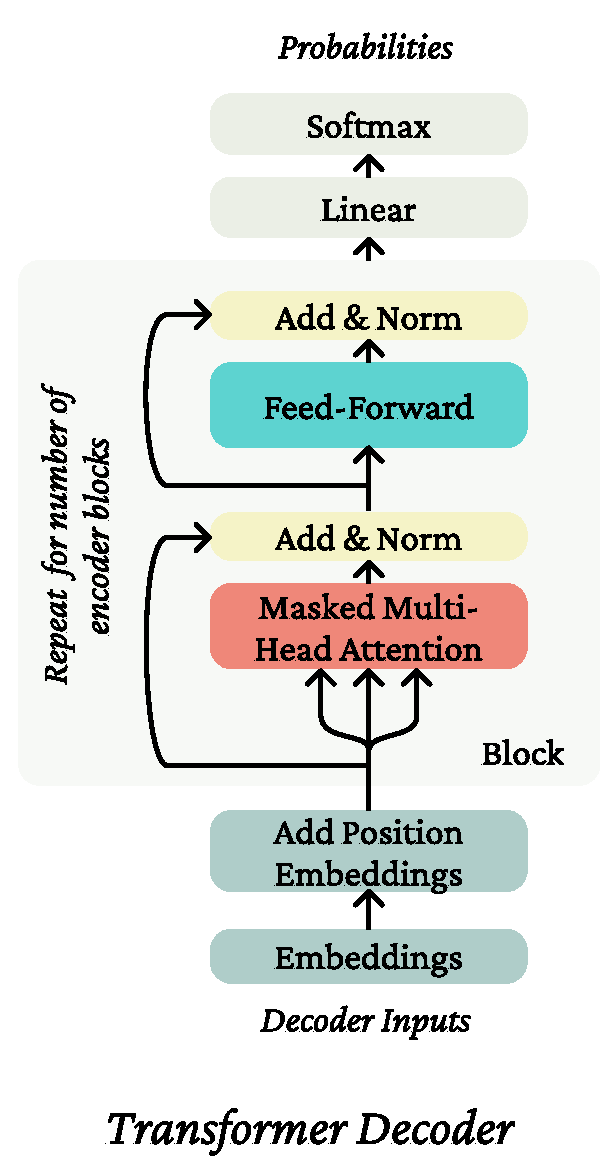
\includegraphics[height=0.6\linewidth]{images/decoder.pdf}
\caption{Illustration of the transformer block.}
\label{fig:tranformer_block}
\end{figure}

The provided \texttt{CausalSelfAttention} layer implements the following attention for each head of the multi-headed attention: Let $X\in \mathbb{R}^{\ell \times d}$ (where $\ell$ is the block size and $d$ is the total dimensionality, $d/h$ is the dimensionality per head.).\footnote{Note that these dimensionalities do not include the minibatch dimension.}

Let $Q_i,K_i,V_i \in \mathbb{R}^{d\times d/h}$.
Then the output of the self-attention head is 
\begin{equation} \label{qkv_eqn}
Y_i = \text{softmax}\bigg(\frac{(XQ_i)(XK_i)^\top}{\sqrt{d/h}}\bigg)(XV_i)
\end{equation}
where $Y_i\in\mathbb{R}^{\ell \times d/h}$.
Then the output of the self-attention is a linear transformation of the concatenation of the heads:
\begin{equation}
Y = [Y_1;\dots;Y_h]A
\end{equation}
where $A \in\mathbb{R}^{d\times d}$ and $[Y_1;\dots;Y_h]\in\mathbb{R}^{\ell \times d}$.
The code also includes dropout layers which we haven't written here.
We suggest looking at the provided code and noting how this equation is implemented in PyTorch.

Our model uses this self-attention layer in the transformer block as shown in Figure~\ref{fig:tranformer_block}. As discussed in the lecture, the transformer block contains residual connections and layer normalization layers. If we compare this diagram with the \texttt{Block} code provided in \texttt{model.py}, we notice that the implementation does not perform layer normalization on the output of the MLP (Feed-Forward), but on the input of the \texttt{Block}. This can be considered equivalent since we have a series of transformer blocks on top of each other. 

In the Perceiver model architecture, we replace the first transformer \texttt{Block} in the model with the \texttt{DownProjectBlock}. This block reduces the length of the sequence from $\ell$ to $m$. This is followed by a series of regular transformer blocks, which would now perform self-attention on the reduced sequence length of $m$. We replace the last block of the model with the \texttt{UpProjectBlock}, which takes in the $m$ length output of the previous block, and projects it back to the original sequence length of $\ell$.

You need to implement the \texttt{DownProjectBlock} in \texttt{model.py} that reduces the dimensionality of the sequence in the first block. To do this, perform cross-attention on the input sequence with a learnable basis $C \in \mathbb{R}^{m \times d}$ as the query, where $m < \ell$. Consequently, Equation~\ref{qkv_eqn} becomes: 

\begin{equation}\label{eqn:down_proj_attn}
Y_i^{(1)} = \text{softmax}\bigg(\frac{(CQ_i)(XK_i)^\top}{\sqrt{d/h}}\bigg)(XV_i)    
\end{equation}

resulting in $Y_i^{(1)} \in\mathbb{R}^{m\times d}$, with $^{(1)}$ denoting that the output corresponds to the first layer. With this dimensionality reduction, the subsequent \texttt{CausalSelfAttention} layers operate on inputs $\in \mathbb{R}^{m\times d}$ instead of $\mathbb{R}^{l\times d}$. We refer to $m$ as the \texttt{bottleneck\_dim} in code. Note that for implementing Equation~\ref{eqn:down_proj_attn}, we need to perform cross attention between the learnable basis $C$ and the input sequence. This has been provided to you as the \texttt{CausalCrossAttention} layer. We recommend reading through \texttt{attention.py} to understand how to use the cross-attention layer, and map which arguments correspond to the key, value and query inputs. Initialize the basis vector matrix $C$ using Xavier Uniform initialization.

To get back to the original dimensions, the last block in the model is replaced with the \texttt{UpProjectBlock}. This block will bring back the output sequence length to be the same as input sequence length  by performing cross-attention on the previous layer's output $Y^{L-1}$ with the original input vector $X$ as the query:

\begin{equation}\label{eqn:up_proj_attn}
Y_i^{(L)} = \text{softmax}\bigg(\frac{(XQ_i)(Y^{(L-1)}K_i)^\top}{\sqrt{d/h}}\bigg)(Y^{(L-1)}V_i)
\end{equation}
where $L$ is the total number of layers. This results in the final output vector having the same dimension as expected in the original \texttt{CausalSelfAttention} mechanism. Implement this functionality in the \texttt{UpProjectBlock} in \texttt{model.py}.



We provide the code to assemble the model using your implemented \texttt{DownProjectBlock} and \texttt{UpProjectBlock}. The model uses these blocks when the \texttt{variant} parameter is specified as \texttt{perceiver}.


Below are bash commands that your code should support in order to pretrain the model, finetune it, and make predictions on the dev and test sets.
Note that the pretraining process will take approximately 2 hours. 
\clearpage
\begin{lstlisting}[basicstyle=\ttfamily, language=bash]

# Pretrain the model
python src/run.py pretrain perceiver wiki.txt --bottleneck_dim 64 \
        --pretrain_lr 6e-3 --writing_params_path perceiver.pretrain.params
        
# Finetune the model
python src/run.py finetune perceiver wiki.txt --bottleneck_dim 64 \
        --reading_params_path perceiver.pretrain.params \
        --writing_params_path perceiver.finetune.params \
        --finetune_corpus_path birth_places_train.tsv
        
# Evaluate on the dev set; write to disk
python src/run.py evaluate perceiver wiki.txt --bottleneck_dim 64 \
        --reading_params_path perceiver.finetune.params \
        --eval_corpus_path birth_dev.tsv \
        --outputs_path perceiver.pretrain.dev.predictions
        
# Evaluate on the test set; write to disk
python src/run.py evaluate perceiver wiki.txt --bottleneck_dim 64 \
        --reading_params_path perceiver.finetune.params \
        --eval_corpus_path birth_test_inputs.tsv \
        --outputs_path perceiver.pretrain.test.predictions
\end{lstlisting}

Report the accuracy of your perceiver attention model on birthplace prediction on \texttt{birth\_dev.tsv} after pretraining and fine-tuning.

Save the predictions of the model on \texttt{birth\_test\_inputs.tsv} to \texttt{perceiver.pretrain.test.predictions}.

For this section, you'll submit: \texttt{perceiver.finetune.params}, \texttt{perceiver.pretrain.dev.predictions},\\ and \texttt{perceiver.pretrain.test.predictions}. Your model should get at least 6\% accuracy on the dev set.
    
\begin{subparts}

\subpart[8]  We'll score your model as to whether it gets at least 5\% accuracy on the test set, which has answers held out.
\begin{figure}[h]
        \centering
        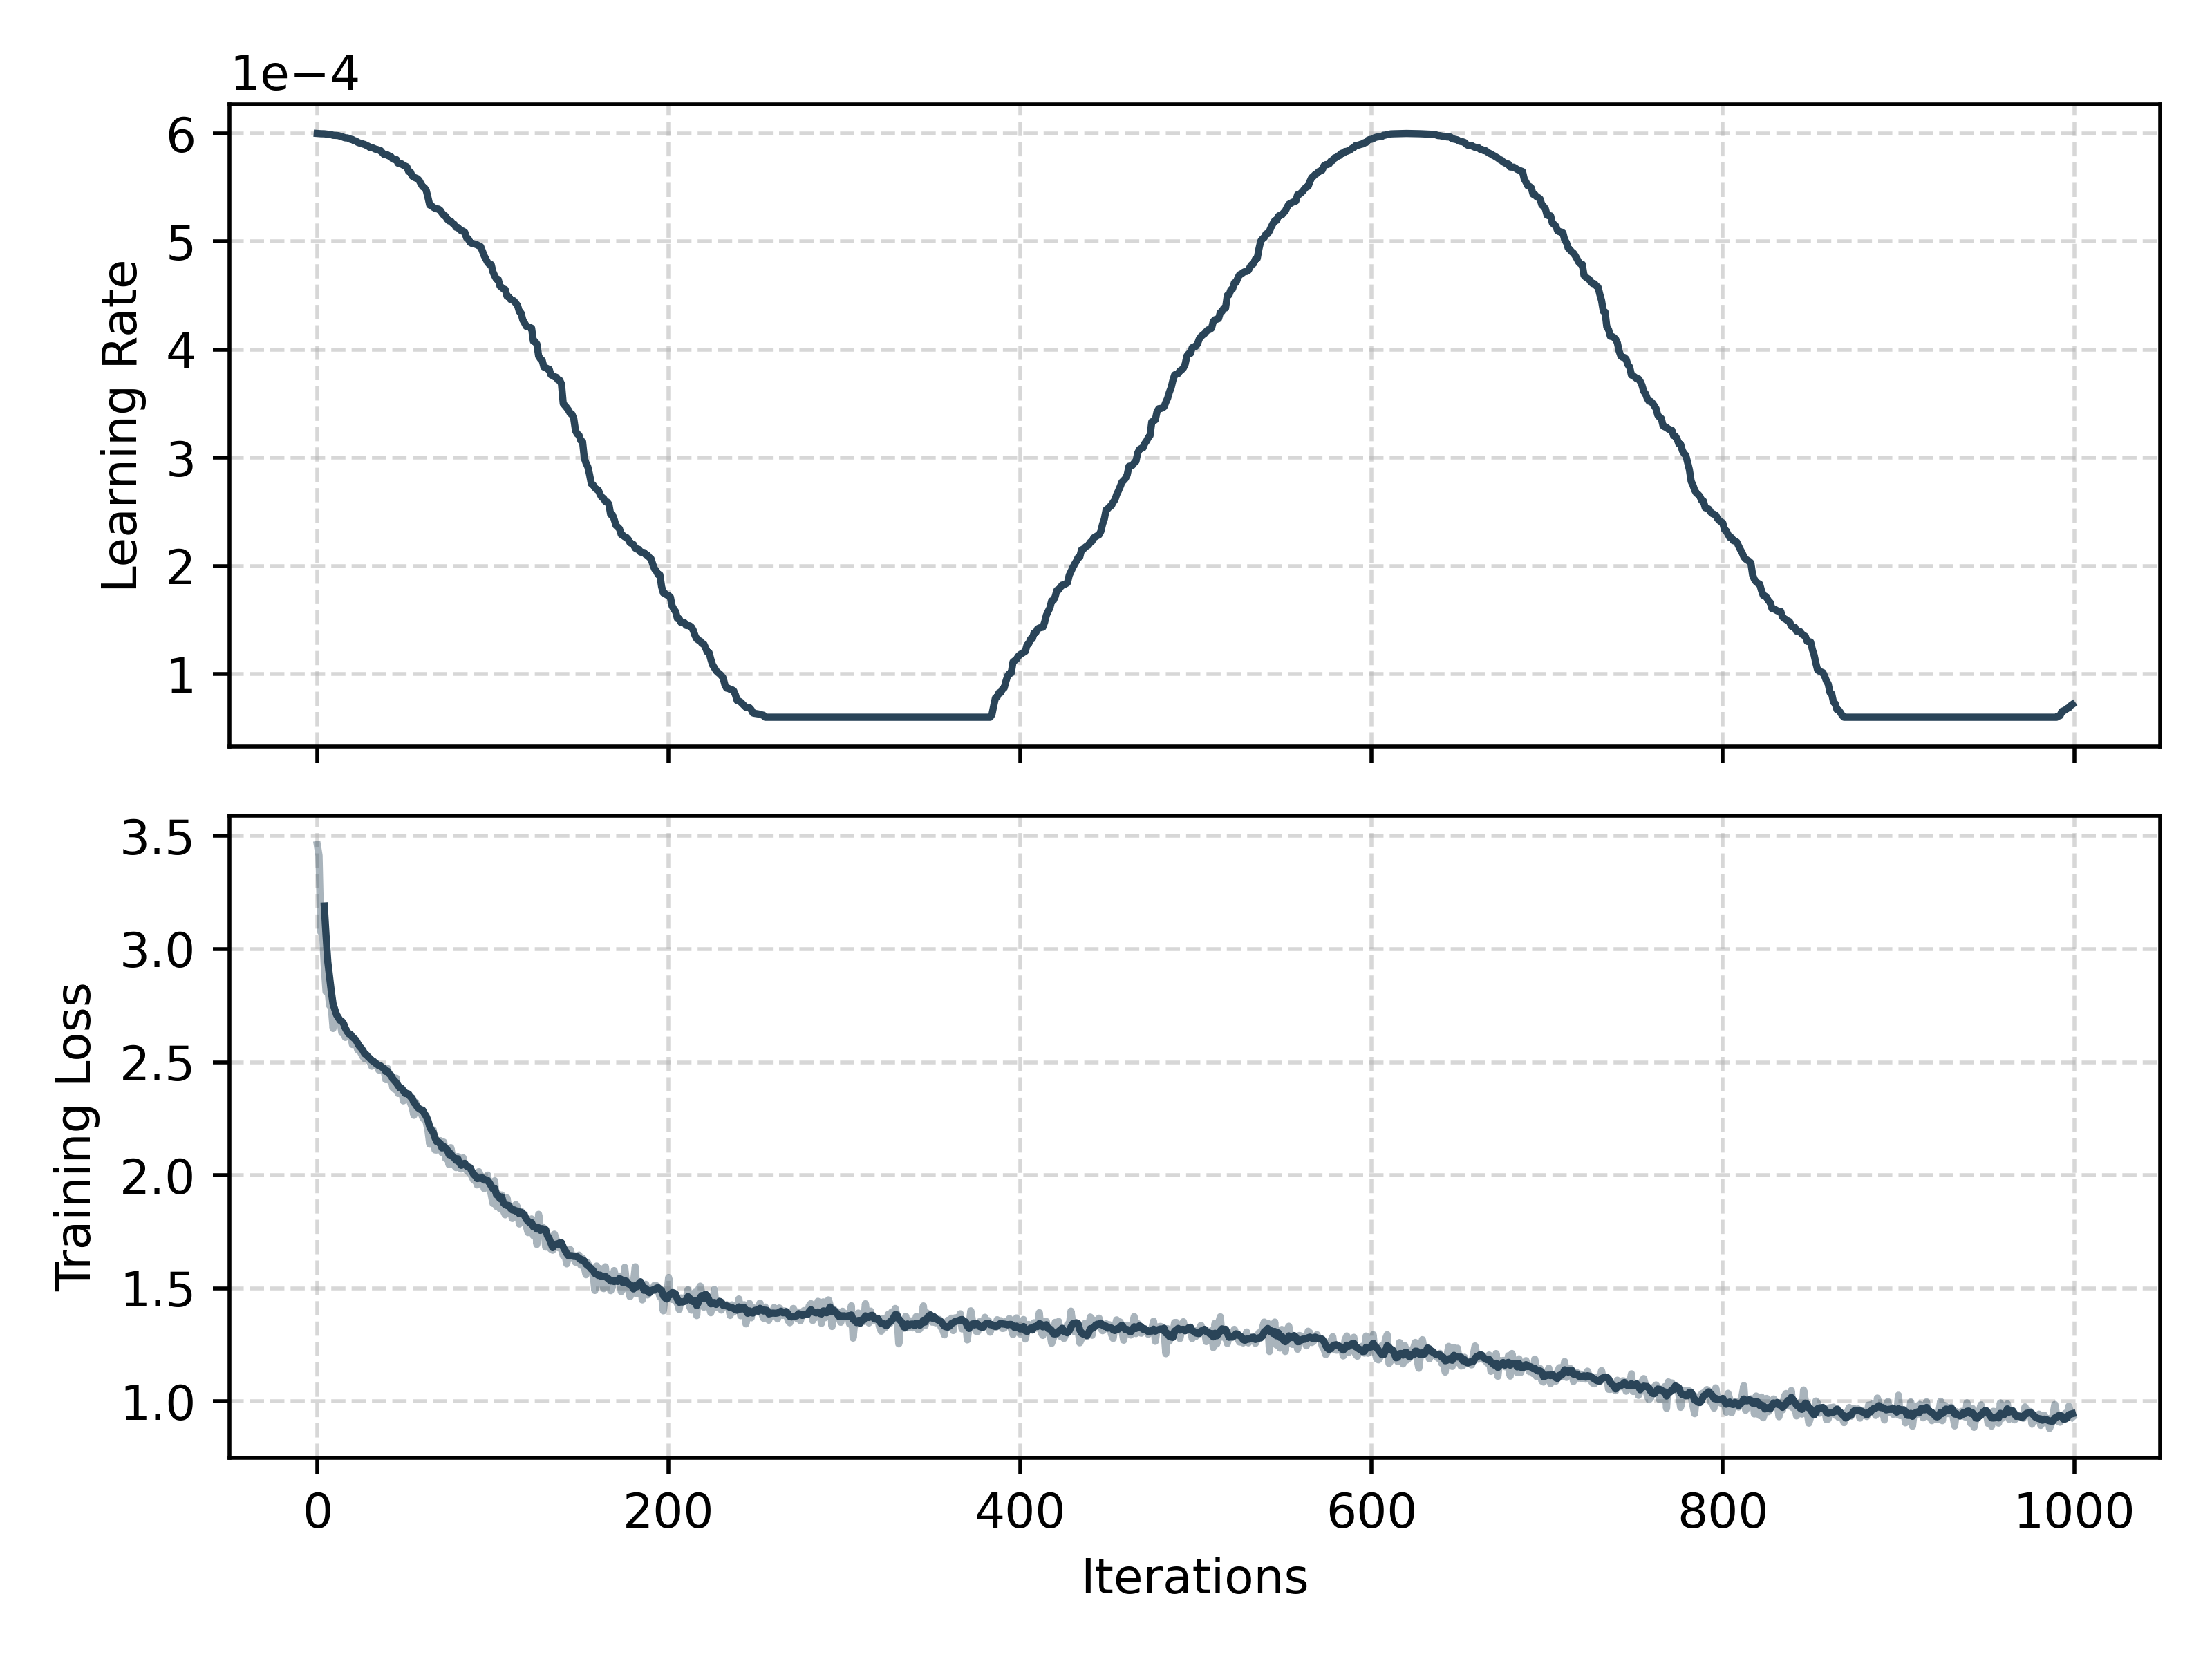
\includegraphics[width=0.5\textwidth]{../code/perceiver_training_process.png}
        \caption{perceiver training process}
        \label{fig:perceiver_training_process}
\end{figure}

\ifans{
        Correct: 40.0 out of 500.0: 8.0\%
}

\subpart[2] Provide an expression for the time complexity of the Perceiver model and the vanilla model, in terms of number of layers ($L$), input sequence length ($\ell$) and basis bottleneck dimension ($m$). 

\ifans{
        \begin{itemize}
                \item Vanilla model: $O(L\ell^2)$, where each layer is self attention layer with complexity $O(\ell^2)$.
                \item Perceiver model: $O(2\ell m + (L-2)m^2)$, where $2$ layers of cross attention for down-projection and up-projection and $L-2$ layers of self attention with complexity $O(m^2)$.
        \end{itemize}
}


\end{subparts}
\end{parts}
\titledquestion{Considerations in pretrained knowledge}[5]
{\color{red} \textbf{Please type the answers to these written questions (to make TA lives easier).}}
\begin{parts}

\part[1] Succinctly explain why the pretrained (vanilla) model was able to achieve an accuracy of above 10\%, whereas the non-pretrained model was not.

\ifans{
        \begin{enumerate}
                \item The pretrained model has been trained on a large corpus of text data, which allows it to learn general language patterns and structures, 
                and gives the model a better ituition about which part is ``person name'', which part is ``birth place'' and how they are related.
                \item The vanilla model is trained on a small dataset, which unable to learn the patterns and structures of ``person name'' and ``birth place''.
                Furthermore, the model cannot handle unseen person names and birth places, which is a common case in the evaluation and test set.
                \item If ``person names'' and ``birth places'' are both have fixed vocabulary and fixed length, the vanilla model may achieve a higher accuracy.
                Because the model can be simplified as a classification model, which can be trained on a small dataset.
        \end{enumerate}
}

\part[2] Take a look at some of the correct predictions of the pretrain+finetuned vanilla model, as well as some of the errors.
We think you'll find that it's impossible to tell, just looking at the output, whether the model \textit{retrieved} the correct birth place, or \textit{made up} an incorrect birth place.
Consider the implications of this for user-facing systems that involve pretrained NLP components.
Come up with two \textbf{distinct} reasons why this model behavior (i.e. unable to tell whether it's retrieved or made up) may cause concern for such applications, and an example for each reason.

\ifans{
        \begin{itemize}
                \item The model may have memorized the association between a person name and a birth place, and may not have learned the underlying patterns in the data. 
                For example: some places are extremely rare, such as ``Brunswick'', ``Canberra'', ``Stuttgart'', ``Wolverhampton'' and ``Milwaukee'' are only mentioned once in the training set, and the model made correct predictions for them.
                The model may have memorized the association between a person name and a birth place, and may not have learned the underlying patterns in the data.
                This may cause concern for applications that require the model to generalize to unseen data.
                \item If the model is used in a user-facing system, the user may not be able to tell whether the model has retrieved or made up the answer. This may cause mislead the user into believing that the model is more accurate than it actually is.
                For example: the model made correct predictions for name-place pairs which are extremely rare in the training set, but if the same name occurs in other places, the model may make wrong predictions.
        \end{itemize}
        
        \begin{tabular}{llrr}
                \toprule
                 & targets & score & count \\
                \midrule
                0 & Athens & 0.333333 & 3 \\
                1 & Baltimore & 0.166667 & 6 \\
                2 & Berlin & 0.166667 & 6 \\
                3 & Brunswick & 1.000000 & 1 \\
                4 & Canberra & 1.000000 & 1 \\
                5 & Charleston & 0.333333 & 3 \\
                6 & Chicago & 0.357143 & 14 \\
                7 & Copenhagen & 0.500000 & 2 \\
                8 & Dresden & 1.000000 & 1 \\
                9 & Dublin & 0.428571 & 7 \\
                10 & England & 0.200000 & 10 \\
                11 & France & 0.333333 & 6 \\
                12 & Frankfurt & 0.500000 & 2 \\
                13 & Glasgow & 0.333333 & 3 \\
                14 & Helsinki & 0.333333 & 3 \\
                15 & Kansas & 1.000000 & 1 \\
                16 & Lawrence & 1.000000 & 1 \\
                17 & Lebanon & 1.000000 & 1 \\
                18 & London & 0.400000 & 25 \\
                19 & Milwaukee & 1.000000 & 1 \\
                20 & Minneapolis & 0.250000 & 4 \\
                21 & Montreal & 0.333333 & 3 \\
                22 & Naples & 0.333333 & 6 \\
                23 & Oslo & 0.333333 & 6 \\
                24 & Ottawa & 0.333333 & 3 \\
                25 & Paris & 0.583333 & 12 \\
                26 & Prague & 0.333333 & 3 \\
                27 & Richmond & 0.500000 & 2 \\
                28 & Rome & 1.000000 & 1 \\
                29 & Savannah & 1.000000 & 1 \\
                30 & Sheffield & 0.250000 & 4 \\
                31 & Stuttgart & 1.000000 & 1 \\
                32 & Sydney & 0.333333 & 6 \\
                33 & Tokyo & 0.500000 & 2 \\
                34 & Toledo & 0.500000 & 2 \\
                35 & Toronto & 0.142857 & 7 \\
                36 & Venice & 0.500000 & 2 \\
                37 & Westminster & 1.000000 & 1 \\
                38 & Wolverhampton & 1.000000 & 1 \\
                \bottomrule
                \end{tabular}
}

\part[2] If your model didn't see a person's name at pretraining time, and that person was not seen at fine-tuning time either, it is not possible for it to have ``learned'' where they lived.
Yet, your model will produce \textit{something} as a predicted birth place for that person's name if asked.
Concisely describe a strategy your model might take for predicting a birth place for that person's name, and one reason why this should cause concern for the use of such applications.
(You do not need to submit the same answer for 3c as for 3b.)

\ifans{
        The model may retrieve a similar or related name from the training data, and output the birth place of that name, or output a birth place according to the context around, or just output a birth place randomly.
        This will generate incorrect predictions for unseen names. 
        Incorrect anwsers is more harmful than no answer, as it may mislead the users behaviors.
}

\end{parts}


